\documentclass[skript.tex]{subfiles}

\begin{document}
\setcounter{chapter}{4}
\setcounter{section}{1}

\textbf{Motivationsfragen:}
\begin{itemize}
	\item Was ist denn oben und was ist unten? (Orientierbarkeit)
	\item Wie sieht es mit Rändern aus, wann sind sie ''glatt'', wann sind sie selbst Mannigfaltigkeiten?
\end{itemize}

\section{Integration auf Mannigfaltigkeiten}
\textbf{Ziel:} Verallgemeinerung des Lebesgue-Integrals auf Mannigfaltigkeiten.

\textbf{Strategie:}
\begin{enumerate}
	\item Nach Definition können wir uns eine Mannigfaltigkeit $M$ lokal mit einer Immersion $\varphi \colon U\sbs\Rn \lra \Rn$ parametrisieren -- also betrachten wir zunächst Stücke von Mannigfaltigkeiten.
	
	\item Eine ''beliebige'' Mannigfaltigkeit zerlegen wir in endlich viele überlappende Teilstücke mit lokalen Parametrisierungen (wir setzen also voraus, dass $M$ einen endlichen Atlas besitzt). Der Wert des Integrals ist unabhängig vom gewählten Atlas. Wichtigstes Hilfsmittel: Partition der Eins.
\end{enumerate}

Zunächst der lineare Fall. Für eine lineare Abbildung $T \colon \R^m \lra \Rn, n\geq m,$ und eine messbare Menge $U\sbs \R^m$ möchten wir den ''m-dimensionalen Flächeninhalt'' von $T(U)$ angeben. Wir erwarten, dass der n-dimensionale ''Flächeninhalt'' von $T(U)$ im Fall $m<n$ Null beträgt\footnote{Siehe \textit{Aufgabe 18}: $\mbb{S}^{n-1}$ ist eine $\lambda^n$-Nullmenge.}.

\begin{lem}
	Sei $T\in\R^{n\times m}$ (charakterisiert lineare Abbildung $\R^m \lra \Rn$) mit Rang $m, n\geq m$. Dann gibt es $Q \in \R^{n\times m}$  und $S \in \R^{m\times m}$ mit $T=QS$, wobei $Q$ eine \textup{Isometrie} ist, das heißt $\abs{Qv}_\Rn = \abs{v}_{\R^m} \forall v \in \R^m$ und $\abs{\det S} = \sqrt{\det T^\tp T }$.
\end{lem}

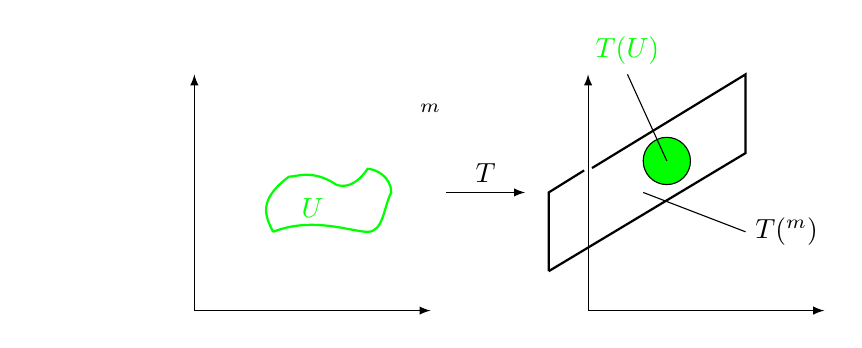
\begin{tikzpicture}
	\node at (-2,0) (nullpunkt) {};
	
	\draw [<->, >=latex] (0,3) -- (0,0) -- (3,0); 
	\draw [green, thick] (1, 1) 
								   .. controls (1.5,1.2) and (2, 1) .. (2.2, 1)
					  			   .. controls (2.4, 1) and (2.4, 1.3) .. (2.5, 1.5)
					  			   .. controls (2.5, 1.7) and (2.3, 1.8).. (2.2, 1.8)
					  			   .. controls (2.0, 1.5) and (1.8, 1.6) .. (1.8, 1.6)
								   .. controls (1.5, 1.8) and (1.3, 1.7) .. (1.2, 1.7)
								   .. controls (0.8, 1.4) and (0.9, 1.2) .. (1,1);
	\node at (1.5, 1.3) (U1)  [green] {$U$};
	\node at (3, 2.5) (Raum1) {$\R^m$};
	
	\draw [->, >=latex] (3.2, 1.5) -- node [above] {$T$} (4.2, 1.5);
	
	\draw [<->, >=latex, thin] (5,3) -- (5,0) -- (8,0);
	\node at (8, 2.5) (Raum2) {$\Rn$};
	\draw [thick] (4.5, 0.5) -- (7,2) -- (7,3) -- (5.05,1.81);
	\draw [thick] (4.95, 1.78) -- (4.5, 1.5) -- (4.5,0.5);
	\draw [fill=green] (6, 1.9) circle [radius=0.3cm];
	\draw (5.7, 1.5) -- (7, 1) node [right] {$T(\R^m)$};
	\draw (6,1.9) -- (5.5, 3) node [above, green] {$T(U)$};
\end{tikzpicture}

\begin{proof}
	Mit $e_1, \dots, e_m$ bezeichnen wir die Standard-Einheitsbasis des $\R^m$. Weiter wählen wir eine Orthonormalbasis $\cbr{f_1, \dots, f_n}$ des $\Rn$ mit $T(\R^m) = \spann \cbr{f_1, \dots, f_m}$.
	
	Nun Können wir $Q \in \R^{n\times m}$ durch $Qe_j = f_j, j=1,\dots,m$ eindeutig definieren und für 
	\[
		v = \sum_{j=1}^{m} v_j e_j,\quad w = \sum_{k =1}^m w_k e_k
	\]
	erhalten wir
	\[
		\skp{Qv}{Qw}_{\Rn} \stackrel{\footnotemark}{=} \sum_{j,k} v_j w_k \delta_{jk} = \sum_{j=1}^m v_j w_j = \skp{v}{w}_{\R^m},
	\]
	\footnotetext{$\skp{f_j}{f_k}_{\R^m} = \delta_{jk}$}
	also $\abs{Qv}_{\Rn} = \abs{v}_{\R^m} \forall\ v\in \R^m$, und
	\[
		\skp{Q^\tp Qv}{w}_{\R^m} = w^\tp Q^\tp Qv = (Qw)^\tp Qv = \skp{Qv}{Qw}_{\Rn} = \skp{v}{w}_{\R^m},
	\]
	woraus $Q^\tp Q = \id_{R^m}$ ersichtlich ist. Nach Konstruktion ist $Q$ auf $T(\R^m)$ invertierbar, somit ist $S \ceq Q^{-1} T \in \R^{m\times m}$ wohldefiniert, und $\rang S = m$. Wir haben $QS = T$ und 
	\begin{align*}
		\det\pr{T^\tp T} = \det\pr{(QS)^\tp QS} &= \det\big( S^\tp \underbrace{Q^\tp Q}_{\mathclap{\id_{\R^m} }} S\big)\\
		&= \det\pr{S^\tp S}\\ 
		&= \det(S) \det\pr{S^\tp}\\
		&= \abs{\det S}^2.
	\end{align*}
\end{proof}

Wir möchten einen ''Flächeninhalt'' definieren, der invariant unter Isometrien (Translation, Rotation, Spiegelung) ist. Insofern sollte der Flächeninhalt von $T(U)$ mit dem von \\$Q^{-1} T(U) = S(U)$ übereinstimmen. Wegen $S(U) \sbs \R^m$ können wir das m-dimensionale Lebesgue-Maß verwenden und erhalten:
\[
	\lambda^m (S(U)) = \lint_{S(U)} \mathds{1} \md \lambda^m \darrow{\textup{I.69c}}{=} \abs{\det S} \lint_U \mathds{1} \md \lambda^m = \sqrt{\det \pr{T^\tp T}} \lambda^m(U).
\]


\begin{defin}[Integral auf lokaler Parametrisierung]
	Seinen $m,n \in \N, m\leq n, U \sbs \Rn$ offen, $\varphi \in \C^1(U,\Rn)$ eine Immersion, die $U$ homöomorph auf $\image \varphi$ abbildet. Dann definieren wir den mehrdimensionalen Flächeninhalt von $\image \varphi$ durch
	\[
		\vol^m(\image \varphi) = \int_U \sqrt{\det \pr{(D\varphi)^\tp (D\varphi)}} \md \lambda^m ,
	\]
	wobei $\det \pr{(D\varphi)^\tp (D\varphi)}$ mit \textit{Gram-Determinante} bezeichnet wird.
	
	Eine Funktion $f\colon \image \varphi \lra \R$ heißt integrierbar, falls
	\[
		(f \circ \varphi) \sqrt{\det \pr{(D\varphi)^\tp (D\varphi)}}
	\]
	auf $U$ integrierbar ist.
	
	Das m-dimensionale Flächenintegral auf $\image \varphi$ ist durch
	\[
		\lint_{\image \varphi} f \md A^m = \lint_U (f\circ \varphi) \sqrt{\det \pr{(D\varphi)^\tp (D\varphi)}} \md \lambda^m
	\]
	gegeben. Entsprechend sind die Räume $L^p (\image \varphi)$ erklärt.
	
	Im Fall $n=m$ ergibt sich mit $\varphi = \id$:
	\[
		\int_U f \md A^n = \int_U f \md \lambda^n.
	\]
\end{defin}

\begin{lem}[Wohldefiniertheit des Flächeninhalts]
	Seien $n,m \in \N, m\leq n, U_1, U_2 \sbs \R^m$ offen und $\varphi_1 \in C^1(U_1, \Rn), \varphi_2 \in C^1(U_2, \Rn)$ Immersionen, die $U_1$ beziehungsweise $U_2$ homöomorph auf eine Menge $W\sbs \Rn$ abbilden. Sei weiterhin $f\colon W \lra \R$ messbar. Dann ist $(f\circ \varphi_1) \sqrt{\det \pr{(D\varphi_1)^\tp (D\varphi_1)}}$ genau dann integrierbar, wenn $(f \circ \varphi_2) \sqrt{\det \pr{(D\varphi_2)^\tp (D\varphi_2)}}$ integriebar ist und wir haben
	\[
		\lint_{U_1} (f \circ \varphi_1) \sqrt{\det \pr{(D\varphi_1)^\tp (D\varphi_1)}} \md \lambda^m = \lint_{U_2} (f\circ \varphi_2) \sqrt{\det \pr{(D\varphi_2)^\tp (D\varphi_2)}} \md \lambda^m.
	\]
\end{lem}

\begin{proof}
	Wir setzen $\psi = \varphi_1^{-1} \circ \varphi_2 \colon U_2 \lra U_1$. Wenn wir zeigen, dass $\psi$ ein Diffeomorphismus ist, so folgt die Behauptung mit dem \textit{Transformationssatz (I.70)} wegen
	\[
		\lint_{U_1} (f\circ \varphi_1) \sqrt{\det \pr{(D\varphi_1)^\tp (D\varphi_1)}} \md \lambda^m = \lint_{U_2} (f\circ \underbrace{\varphi_1 \circ \psi)}_{\varphi_2} \sqrt{\det \pr{(D\varphi_1 \circ \psi)^\tp (D\varphi_1 \circ \psi)}} \abs{\det D\psi} \md \lambda^m,
	\]
	woraus wir mit $D\varphi_2 = D(\varphi_1 \circ \psi) = (D\varphi_1 \circ \psi) D\psi$ und
	\begin{align*}
		\det \pr{(D\varphi_2)^\tp (D\varphi_2)} &= \det \big( (D\psi)^\tp \underbrace{(D\varphi_1 \circ \psi)^\tp (D\varphi_1 \circ \psi)}_{\in \R^{m\times m}} (D\psi) \big)\\
		&= \det (D\psi) \det \pr{(D\varphi_1 \circ \psi)^\tp (D\varphi_1 \circ \psi)} \det (D\psi)\\
		&= \abs{\det D\psi}^2 \det \pr{(D\varphi_1 \circ \psi)^\tp (D\varphi_1 \circ \psi)}
	\end{align*}
	die geforderte Identität erhalten.
	
	Es bleibt zu zeigen, dass $\psi$ ein Diffeomorphismus ist. Als Verkettung zweier Homöomorphismen ist $\psi$ wieder ein Homöomorphismus. Insofern genügt der Nachweis, dass $\psi, \psi^{-1} \in C^1$ sind. Aus Symmetriegründen können wir uns auf $\psi \in C^1$ beschränken. 
	
	Zur Charakterisierung von $\varphi_1^{-1}$ fixieren wir ein beliebiges $u_2 \in U_2$ und setzen $x=\varphi_2(u_2),\\u_1=\varphi_1^{-1}(x) = \psi(u_2)$. Die Spalten von $D\varphi_1(u_1)$ spannen den Tangentialraum $T_x W$ an $W$ im Punkt $x$ auf. Mit $P$ bezeichnen wir die Projektion $P\colon \Rn \lra T_x W \cong \R^m$. Nach der Kettenregel haben wir für $P \circ \varphi_1 \colon U_1 \lra T_x W$
	\[
		D(P\circ \varphi_1)(u_1) = DP\big( \underbrace{\varphi_1(u_1)}_{x} \big) D\varphi_1(u_1) = P\pr{D\varphi_1(u_1)} = D\varphi_1(u_1).
	\]
	Insbesondere ist $\rang D(P\circ\varphi_1)(u_1) = \rang D\varphi_1(u_1) = m$.
	
	Nach dem Umkehrsatz ist $P\circ \varphi_1$ in einer Umgebung von $u_1$ invertierbar. Folglich gibt es Umgebungen $\wt{U}_1 \sbs \R^m, \wt{W} \sbs T_x W$ mit $u_1 \in \wt{U}_1$ und $g \in C^1(\wt{W}, \wt{U}_1)$ mit $g \circ P \circ \varphi_1 = \id_{\wt{U}_1}$. Wir setzen $\wt{U}_2 = \varphi_2^{-1}(\wt{W})$ und erhalten $\psi = \varphi_1^{-1} \circ \varphi_2 = g \circ P \circ \varphi_2$ auf $\wt{U}_2$. Insbesondere ist $\psi|_{\wt{U}_2} \in C^1(\wt{U}_2, \R^m)$. Da $u_2$ beliebig war, folgt $\psi \in C^1(U_2, \R^m)$.
\end{proof}
\end{document}